%%
%% copyright quintard julien
%%
%% kaneton
%%
%% design.tex
%%
%% path          /home/ultima/g/kaneton/view/cursus/schedule
%%
%% made by mycure
%%         quintard julien   [quinta_j@epita.fr]
%%
%% started on    Fri Feb  4 15:10:05 2005   mycure
%% last update   Sun Dec 11 02:27:59 2005   cedric
%%

%
% template
%

%
% ---------- header -----------------------------------------------------------
%
% project       kaneton
%
% license       kaneton
%
% file          /home/mycure/kaneton/view/template/paper.tex
%
% created       julien quintard   [wed may 16 18:17:37 2007]
% updated       julien quintard   [fri oct  5 07:00:45 2007]
%

%
% class
%

\documentclass[10pt,a4wide]{article}

%
% packages
%

\usepackage[english]{babel}
\usepackage[T1]{fontenc}
\usepackage{a4wide}
\usepackage{fancyheadings}
\usepackage{multicol}
\usepackage{indentfirst}
\usepackage{graphicx}
\usepackage{color}
\usepackage{xcolor}
\usepackage{verbatim}
\usepackage{aeguill}

\pagestyle{fancy}

\setlength{\footrulewidth}{0.3pt}
\setlength{\parindent}{0.3cm}
\setlength{\parskip}{2ex plus 0.5ex minus 0.2ex}

%
% logos
%

\newcommand{\logos}
  {
    \begin{center}
      
\includegraphics[scale=0.8]{\path/logo/kaneton.pdf}
    \end{center}
  }

%
% prototype
%

\newcommand\prototype[2]{
  \begin{tabular}{p{0.2cm}p{13.8cm}}
  & #1
  \end{tabular}

  \begin{tabular}{p{1cm}p{13cm}}
  & #2
  \end{tabular}}

%
% verbatim stuff
%

\definecolor{verbatimcolor}{rgb}{0.00,0.40,0.00}

\makeatletter

\renewcommand{\verbatim@font}
  {\ttfamily\footnotesize\selectfont}

\def\verbatim@processline{
  {\color{verbatimcolor}\the\verbatim@line}\par
}

\makeatother

%
% header
%

\rhead{}
\rfoot{\scriptsize{The kaneton microkernel project}}

\date{\scriptsize{\today}}


%
% header
%

\lhead{\scriptsize{The kaneton project scheduling}}

%
% title
%

\title{The kaneton microkernel project}

%
% authors
%

\author{\small{Julien Quintard}}

%
% document
%

\begin{document}

%
% title
%

\maketitle

%
% --------- text --------------------------------------------------------------
%

\begin{multicols}{2}


%
% overview
%

\section{Overview}

\textbf{kaneton} is a project of the EPITA specialisation year in system,
network and security.

The goal of the project is to give students a complete view of an operating
system.

Every group, composed of about four students, has to develop parts
of the kaneton microkernel.

To do so, the professors give students a development environment containing
everything needed to start the project.

The whole project is divided into parts, each part must be validated by
the students.

The project comes with four, maybe five, courses:

\begin{itemize}
  \item
    \textbf{kaneton}: this course is intended to give students a good overview
    of operating system design problems and introduced the kaneton design.
  \item
    \textbf{kernel}: this course give a complete study of the kernel
    internals including microkernels, memory management, processes and threads,
    synchronisation, communications, and complete case studies.
  \item
    \textbf{mips architecture}: this course is dedicated to the mips internal
    architecture including the pipeline, the bus etc..
  \item
    \textbf{intel 32-bit architecture}: this course will explain the Intel
    external architecture including the instructions sets, the
    memory management and finally to the task management.
  \item
    \textbf{distributed operating system}: this course is intented to
    give students a simple approach of the distributed inherent problems.
\end{itemize}

Let's see the year scheduling:

\begin{itemize}
  \item
    \textbf{k0}: the students will have to learn low-level programming to
    understand the external architecture programming interface and the
    different memory management models. This part is called the bootstrap.
  \item
    \textbf{k1}: the students will develop a bootloader. Its role is to
    build a memory environment for the futur kernel execution. In this
    project, the students will learn to deal with the virtual memory
    and to develop in a very strict environment, from scratch.
  \item
    \textbf{k2}: this project will lead the students to an higher abstraction
    level. The goal of the project is to develop parts of the set manager,
    the id manager, the address space manager and finally the segment
    manager to be able to manage physical memory.
  \item
    \textbf{k3}: this project introduces the development of some drivers
    (console, keyboard, demonstration shell) and the development of the
    region manager to provide virtual memory operations. Moreover the
    students will have to implement the generic events interface.
  \item
    \textbf{k4}: the students will have to develop the task manager, the
    thread manager and the scheduler to provide the kaneton microkernel
    the possibility to create execution contexts.
  \item
    \textbf{k5}: this project introduces the communication into the
    microkernel and some microkernel servers.
  \item
    \textbf{kn}: this project is a free one. Each group has to choose the
    subject of this project, to design, to implement and to document
    the project. The themes for this project are: distributed aspects,
    security or network. Some subjects will be proposed to the best groups.
\end{itemize}



%
% arch-mips
%

\section{arch-mips}

\textit{Name}: \textbf{MIA}

\textit{Hours}: \textbf{30 hours} divided into \textbf{10 sessions}

\textit{Professor}: \textbf{Julien Quintard}

This course is intended to give students a complete view of how a RISC
processor works and what choices the designers made to build the futur
processors.

\begin{itemize}
  \item
    External architecture: we will study the instructions set,
    the memory management model etc..
  \item
    Pipeline: we will study the MIPS pipeline, its inherent problems
    and limitations.
  \item
    Compiler optimisations: we will study the different direct assembly
    source code optimisations: rescheduling, software pipelining etc..
  \item
    Memory: we will study the bus used on the MIPS processor and
    the different cache management techniques.
\end{itemize}

The list below details the different sessions for the mips architecture
course:

\begin{enumerate}
  \item
    Course presentation, MIPS history, introduction to MIPS external
    architecture: registers and instructions set. Introduction to
    instruction formats and to inherent limitations. (3 hours)
  \item
    End of instruction formats introduction, explanations of architecture
    designers choices: MIXs and Amdhal Rule. Some exercises to practice.
    Introduction to MIPS architecture addressing and to MIPS pipeline.
    (3 hours)
  \item
    Introduction to MIPS spirit and to its pipeline. Moore Law and
    pipeline rules. Introduction to different pipeline representations:
    simplified and detailed. Some exercises to pratice these representations.
    (3 hours)
  \item
    We will study in this session the next instruction address computation
    problem and the delay slot. Then, study of branch instruction and their
    problems and limitations. Some exercises to pratice. (3 hours)
  \item
    Complete study of instruction dependencies. Some exercise to practice.
    Introduction to optimisations. (3 hours)
  \item
    Study of different optimisations used by compilers. Study of
    advanced pipelines: superpipeline, superscalar etc.. (3 hours)
  \item
    Introduction to the Pi Bus used by MIPS microprocessor. Then complete
    study of memory including cache management. (3 hours)
  \item
    End of memory course. Some exercises to practice. (3 hours)
  \item
    Revisions. (3 hours)
  \item
    Padding course. (3 hours)
\end{enumerate}



%
% kaneton
%

\section{kaneton}

\textit{Name}: \textbf{KAN}

\textit{Hours}: \textbf{35 hours}

\textit{Professor}: \textbf{Julien Quintard}

\textit{Assistants Professor}: \textbf{Cedric Aubouy},
                               \textbf{Renaud Lienhart}

This course will provide students a complete view of an operating system.
Moreover this courses is coupled with a project which consists in the
development of parts of a microkernel.

\begin{itemize}
  \item
    XXX
\end{itemize}

The list below details the different sessions for the kaneton course.

\begin{enumerate}
  \item
    Project presentation: professors, projects, schedule, design overview
    etc.. (2 hours)
  \item
    Languages prerequisites for the kaneton project. (2 hours)
  \item
    \textbf{k0} project presentation. This project must be delivered by
    each group \textbf{two weeks} after the publication of the
    subject. (1 hour)
  \item
    TP for the k0 project about \textbf{three days} after the publication of
    the subject. (3 hours)
  \item
    \textbf{k1} project presentation. This project must be delivered
    \textbf{three weeks} afther the publication of the subject. (2 hours)
  \item
    Development environment presentation to lead students to a better
    comprehension of the kaneton development environment including scripts,
    organisation, makefiles etc.. (2 hours)
  \item
    TP for the k1 project during the first week of the project so about
    \textbf{three days} after the subject's publication. (2 hours)
  \item
    TP for the k1 project during the second week of the project so
    \textbf{in the middle of the second week}. (3 hours)
  \item
    Advanced makefiles presentation to lead students to a better
    comprehension of the kaneton building system. (3 hours)
  \item
    TP for the k1 project during the third week of the project so about
    \textbf{four days} before the end of the project. (3 hours)
  \item
    \textbf{k2} project presentation. This project must be delivered
    in the next \textbf{two weeks}. (2 hours)
  \item
    C-preprocessor presentation to lead students to perfectly understand
    the kaneton core set manager. (2 hours)
  \item
    \textbf{k3} project presentation. This project must be delivered
    \textbf{two weeks} after the subject's publication. (2 hours)
  \item
    TP for the k3 project \textbf{during the second week} so in the
    middle of this week. (2 hours)
  \item
    \textbf{k4} project presentation. This project must be delivered
    \textbf{XXX weeks} after the publication of the project. (2 hours)
  \item
    \textbf{k5} project presentation. The project must be delivered
    \textbf{XXX weeks} after the publication of the project. (2 hours)
  \item
    \textbf{kn} XXX
\end{enumerate}



%
% arch-ia32
%

\section{arch-ia32}

\textit{Name}: \textbf{INA}

\textit{Hours}: \textbf{16 hours}

\textit{Professor}: \textbf{Renaud Lienhart}

This course will explain how the intel 32-bit architecture works including
the memory management, the task management, the instructions set, the
interruption and exception management etc..

\begin{itemize}
  \item
    XXX
\end{itemize}

The list below details the different sessions for the intel 32-bit
architecture course.

\begin{enumerate}
  \item
    XXX
\end{enumerate}



%
% noyau
%

\section{kernel}

\textit{Name}: \textbf{KER}

\textit{Hours}: \textbf{20 hours} divided into \textbf{10 sessions}

\textit{Professor}: \textbf{Cedric Aubouy}

This course is intended to give the students a general overview of
kernel internals and its problematics. It will end with an examination to
evaluate their understanding of the courses and their ability to
conceive and argue coherent system solutions of their own.

The projected planning of the different sessions for the kernel
course is (currently not enough detailed, will be completed later):
\begin{enumerate}
  \item \textbf{micro-kernel:} quick introduction to the courses. Overview
  of kernel history and trends. Birth and evolution of micro-kernels, their
  fundamentals.
  \item \textbf{memory management:} hardware base of memory management. What
  kind of resulting constraints ? Physcical and virtual memory management.
  \item \textbf{processes & threads:} current kernels manage simultaneous
  executions. What kind of solutions to handle them ?
  \item \textbf{synchronisation:} concurrent access to shared resources is a
  common problem in all levels of multithreaded kernels. How to resolve it,
  famous case studies.
  \item \textbf{communication (IPC):} quick overview of communications forms
  from signals to message passing. New problems in the security and shape of
  IPC, introduced by the micro-kernel design.
  \item \textbf{case studies:} projected studies on Hurd, L4 and Mach, but still
  to confirm.
\end{enumerate}




\end{multicols}

\begin{figure}[h]
\centerline{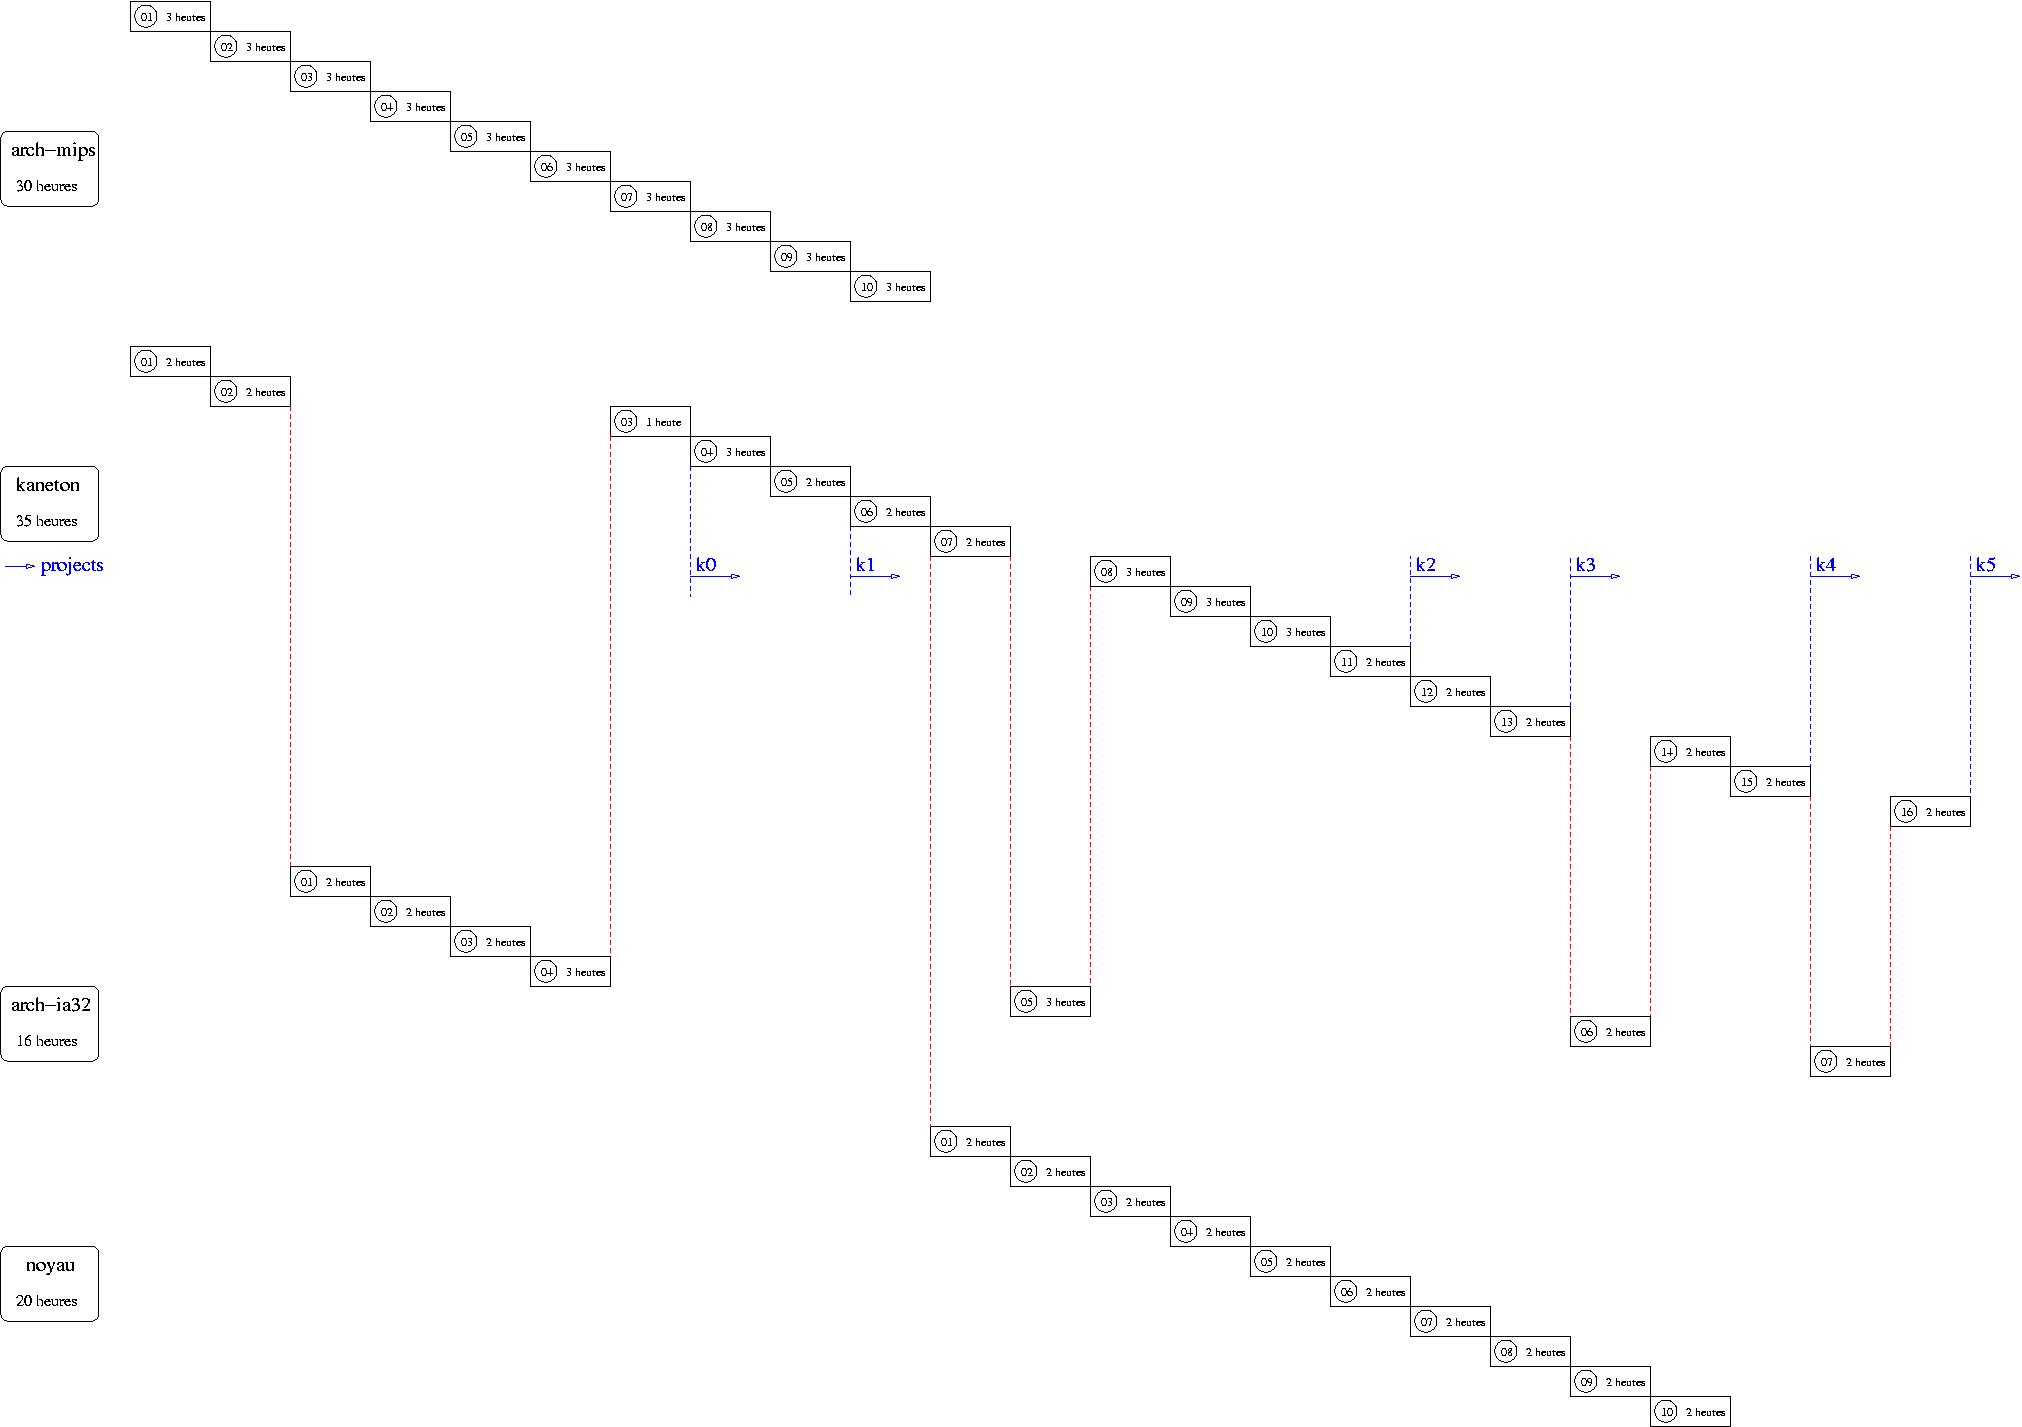
\includegraphics[angle=-90,scale=0.3]{figures/schedule.jpg}}
\end{figure}

\end{document}
